% Part: history
% Chapter: set-theory
% Section: limits

\documentclass[../../../include/open-logic-section]{subfiles}

\begin{document}

\olfileid{his}{set}{limits}	

\olsection{د حدونو کره تعريف}

نن سبا د پورتنۍ مسئلې معياري حل د انفينټېسيمالونو پرېښودل دي۔ دا يې طريقه ده۔

ومو ليدل چې څومره $\beta$ کوچنے کېږي، د ميلان هومره ښه تقريبونه ترلاسه کوو۔ په رښتيا، چې $\beta$ له $0$ سره هر څومره نژدې کېږي، د $f'(c)$ ارزښت هغه ميلان ته «بې له حده ورنژدې کېږي» چې موږ يې غواړو۔ نو د دې پر ځای چې د $\beta = 0$ \emph{په حالت کښې} پېښې په پام کښې ونيسو، يوازې د $f'(c)$ \emph{بهير} په پام کښې نيولو ته اړتيا لرو، کله چې $\beta$ له $0$ سره نژدې کېږي۔ \emph{سرچينه‌يي يادونه OLSTH-047: په دې پاراګراف کښې د ثابتې نقطې مشتق د بدلېدونکي تقريب لپاره کارول شوے دے۔ بدلېدونکے مقدار په پورتنۍ برخه کښې د تابع د ارزښتونو د توپير نسبت دے؛ د ثابتې تابع او ثابتې نقطې مشتق، که موجود وي، يو ثابت ارزښت لري۔ اصلي نښه‌ليکنه ساتل شوې، او دلته د مشتق او د هغه د تقريب توپير څرګند شو۔}

په دې ډول چې يې ووايو، عمومي ستونزه د داسې دعوو په معنا پوهېدل دي:
\begin{center}
چې $x$ له $c$ سره نژدې کېږي، $g(x)$ له $\ell$ سره بې له حده نژدې کېږي۔
\end{center}
دا په لا لنډه بڼه داسې ليکلے شو:
\[
\lim_{x \rightarrow c}g(x) = \ell.
\]
په 19مه پېړۍ کښې وايرشټراس، د کوشي د پخواني کار پر بنسټ، د دې عبارت يو پوره کره تعريف وړاندې کړ۔ نظر دا دے چې $g(x)$ له~$\ell$ سره هر څومره چې وغواړو نژدې کولے شو، که $x$ له~$c$ سره په مناسبه توګه نژدې کړو۔ په لا کره توګه، دا ټاکو چې
$\lim_{x \rightarrow c} g(x) = \ell$ به دا معنا لري:
\[
(\forall\epsilon > 0)(\exists \delta > 0)\forall x \left(|x - c| < \delta \lif |g(x) - \ell| < \epsilon \right).
\]
\emph{سرچينه‌يي يادونه OLSTH-048: د تابع د حد په معمول تعريف کښې نژدې کېدونکے دليل بايد له مرکزي نقطې سره برابر نۀ وي؛ د چاپي شرط د واټن مثبتوالے پاتې دے۔ چاپي فارمول ساتل شوے، خو په همدغه بڼه د مرکزي نقطې ارزښت هم پر حد تحميلوي۔ مثلاً که تابع په صفر کښې يو وي او په ټولو نورو نقطو کښې صفر وي، نو په صفر کښې يې معمول حد صفر دے، خو چاپي شرط د نيم واحد دقت لپاره نۀ پوره کېږي۔ د مشتق د توپير نسبت هم په صفر زياتوالي کښې نۀ دے تعريف شوے؛ د حد اخيستنه يې د صفر پرته پر نژدې دليلونو ده۔}
دلته عمودي کرښې مطلقه اندازه ښيي۔ يعنې $|x| = x$ که $x \geq 0$ وي، او $|x| =-x$ که $x < 0$ وي؛ \emph{دا} تابع داسې ښودلے شئ:
\begin{center}
	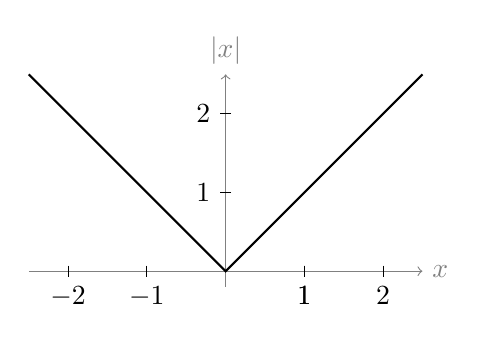
\begin{tikzpicture}[scale=1]
	\draw[->, gray] (-2.5,0) -- (2.5,0) node[right] {$x$};
	\draw[->, gray] (0,-.2) -- (0,2.5) node[above] {$|x|$};

	\foreach \x/\xtext in {-2/-2, -1,1, 1/1, 2/2}
	\draw[shift={(\x,0)}] (0pt,2pt) -- (0pt,-2pt) node[below] {{$\xtext$}};

	\foreach \y/\ytext in {1/1, 2/2}
	\draw[shift={(0,\y)}] (2pt,0pt) -- (-2pt,0pt) node[left] {{$\ytext$}};

	\draw[thick] (-2.5, 2.5)--(0,0)--(2.5, 2.5);
	\end{tikzpicture}
\end{center}
نو تعريف تقريباً دا وايي: خپل «خطا» له $\epsilon$ څخه کمه کولے شئ (يعنې $|g(x) - \ell| < \epsilon$)، که داسې دليلونه وټاکئ چې له $\delta$ څخه زيات واټن د~$c$ څخه ونۀ لري (يعنې $|x -
c| < \delta$)۔

چې د حد مفهوم مو تعريف کړ، نو د انفينټېسيمالونو د پوره پرېښودلو لپاره يې کارولے شو، او دا ټاکلے شو چې د $f$ ميلان په $c$ کښې داسې راکول کېږي:
\[
{f}'(c) = \lim_{x \rightarrow 0}\left(\frac{f(c +x) - f(c)}{x}\right) \text{ چې حد موجود وي}.
\]
خو دا پوهېدل مهم دي چې ولې زموږ تعريف د «چې حد موجود وي» قيد ته اړتيا لري۔ د يوې ساده بېلګې لپاره $f(x) = |x|$ په پام کښې ونيسئ، چې ګراف مو يې اوس وليد۔ ښکاره ده چې $f'(0)$ سم نۀ دے تعريف شوے: که له «ښي لوري» $0$ ته نژدې شو، ميلان تل $1$ وي؛ که له «کيڼ لوري» $0$ ته نژدې شو، ميلان تل $-1$ وي؛ نو حد نۀ دے تعريف شوے۔ له دې امله زياتولے شو چې يوه تابع~$f$ په~$x$ کښې \emph{د مشتق اخيستلو وړ} ده که او يوازې که داسې حد موجود وي۔

ومو ليدل چې د \emph{حد} په مفهوم څنګه مشتق اخيستل سمبال کړو۔ همدغه مفهوم د \emph{پيوستې} تابع د نظر د تعريف لپاره کارولے شو۔ (بولڅانو تر 1817 پورې په اصل کښې دا درک کړے و۔) د پيوستون په اړه د کوشي--وايرشټراس طريقه دا ده۔ په لنډه توګه: يوه تابع~$f$ (په يوه نقطه کښې) پيوسته ده، که د تابع د راوتلي ارزښت لپاره د يو ټاکلي دقت غوښتنه په دې تضمين کړے شئ چې د تابع د داخلېدونکي دليل لپاره پر يو ټاکلي دقت ټينګار وکړئ۔ په لا کره توګه: $f$ په $c$ کښې پيوسته ده، که، چې $x$ صفر ته ورنژدې کېږي، د $f(c + x)$ او $f(c)$ توپير خپله $0$ ته ورنژدې شي۔ په نورو ټکو: $f$ په $c$ کښې \emph{پيوسته} ده که او يوازې که $f(c) = \lim_{x \rightarrow c} f(x)$ وي۔

نور وړاندې تګ به مو حقيقي تحليل ته بوځي، حال دا چې زموږ موضوع سټ نظريه ده۔ نو اوس بايد تم شو او حاصل يې بيان کړو۔ په 19مه پېړۍ کښې رياضيپوهانو زده کړل چې د \emph{حد} د کره تعريف شوي مفهوم په کارولو څنګه له انفينټېسيمالونو پرته کار وکړي۔

\end{document}
